\documentclass[10pt, aspectratio=169]{beamer}

\usetheme[progressbar=frametitle]{metropolis}
\usepackage{appendixnumberbeamer}

\usepackage{booktabs}
\usepackage[scale=2]{ccicons}

\usepackage{pgfplots}
\usepgfplotslibrary{dateplot}

\usepackage{xspace}

\usepackage{changepage}
\usepackage{multicol}

\title{Generation of a Synthetic Population and Travel Network for an Agent Based Traffic Simulation}
\author{Aniruddh Mishra}
\date{August 4, 2023}
\institute{Institute for Computing in Research}

\begin{document}

    \maketitle
    
    \begin{frame}{Table of contents}
        \begin{adjustwidth}{3em}{-1em}
            \setbeamertemplate{section in toc}[sections numbered]
            \begin{multicols}{2}
                \setlength{\parskip}{2em}
                \tableofcontents
            \end{multicols}
        \end{adjustwidth}
    \end{frame}
    
    \section{Introduction}
    
    \begin{frame}[fragile]{Goals}
        \begin{center}
            \begin{figure}
                \centering
                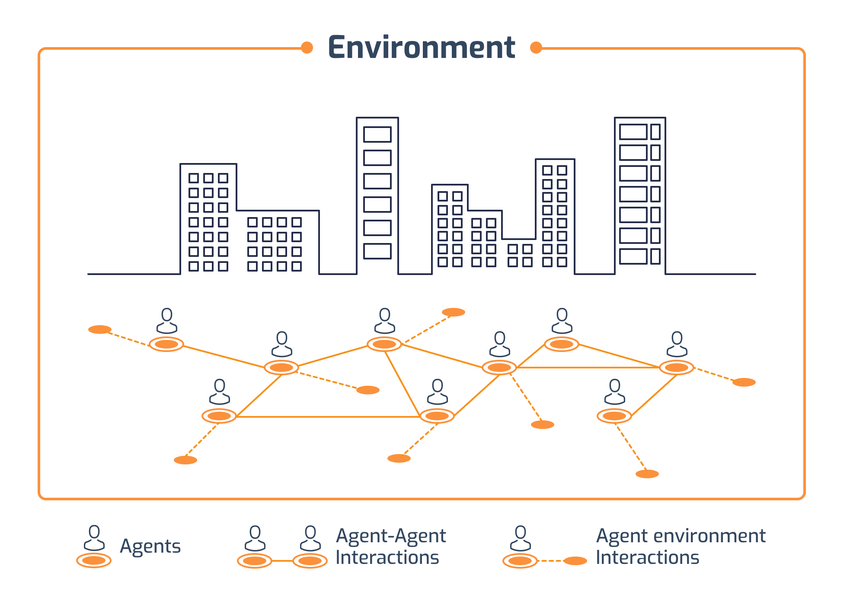
\includegraphics[height=5.5cm, keepaspectratio]{images/agent-based-model.png}
                \caption{Agent Based Model Diagram \cite{agentbasedmodel}}
            \end{figure}
        \end{center}
        % Make Agent Based Model Input
        % Modular Synthesis of this demand
        % Experimental Trials on Generated Demand
    \end{frame}
    
    \begin{frame}[fragile]{Traffic Modeling}
        \begin{center}
            \begin{figure}
                \centering
                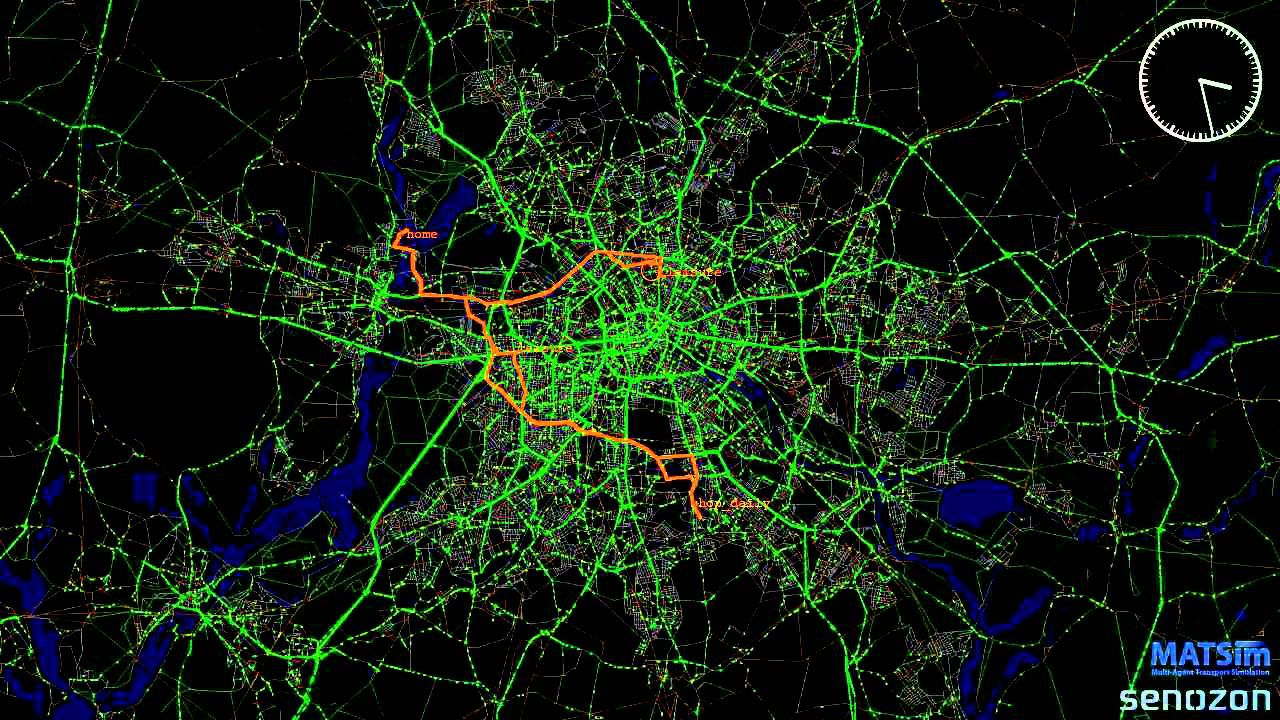
\includegraphics[height=5cm, keepaspectratio]{images/senozon.jpeg}
                \caption{Senozon Visualization of MATSIM Model \cite{senozon}}
            \end{figure}
        \end{center}
        % Why agent based modeling over aggregate modeling?
        % Traffic Demand Generation
    \end{frame}
    
    \begin{frame}{Île-de-France}
        \begin{center}
            \begin{figure}
                \centering
                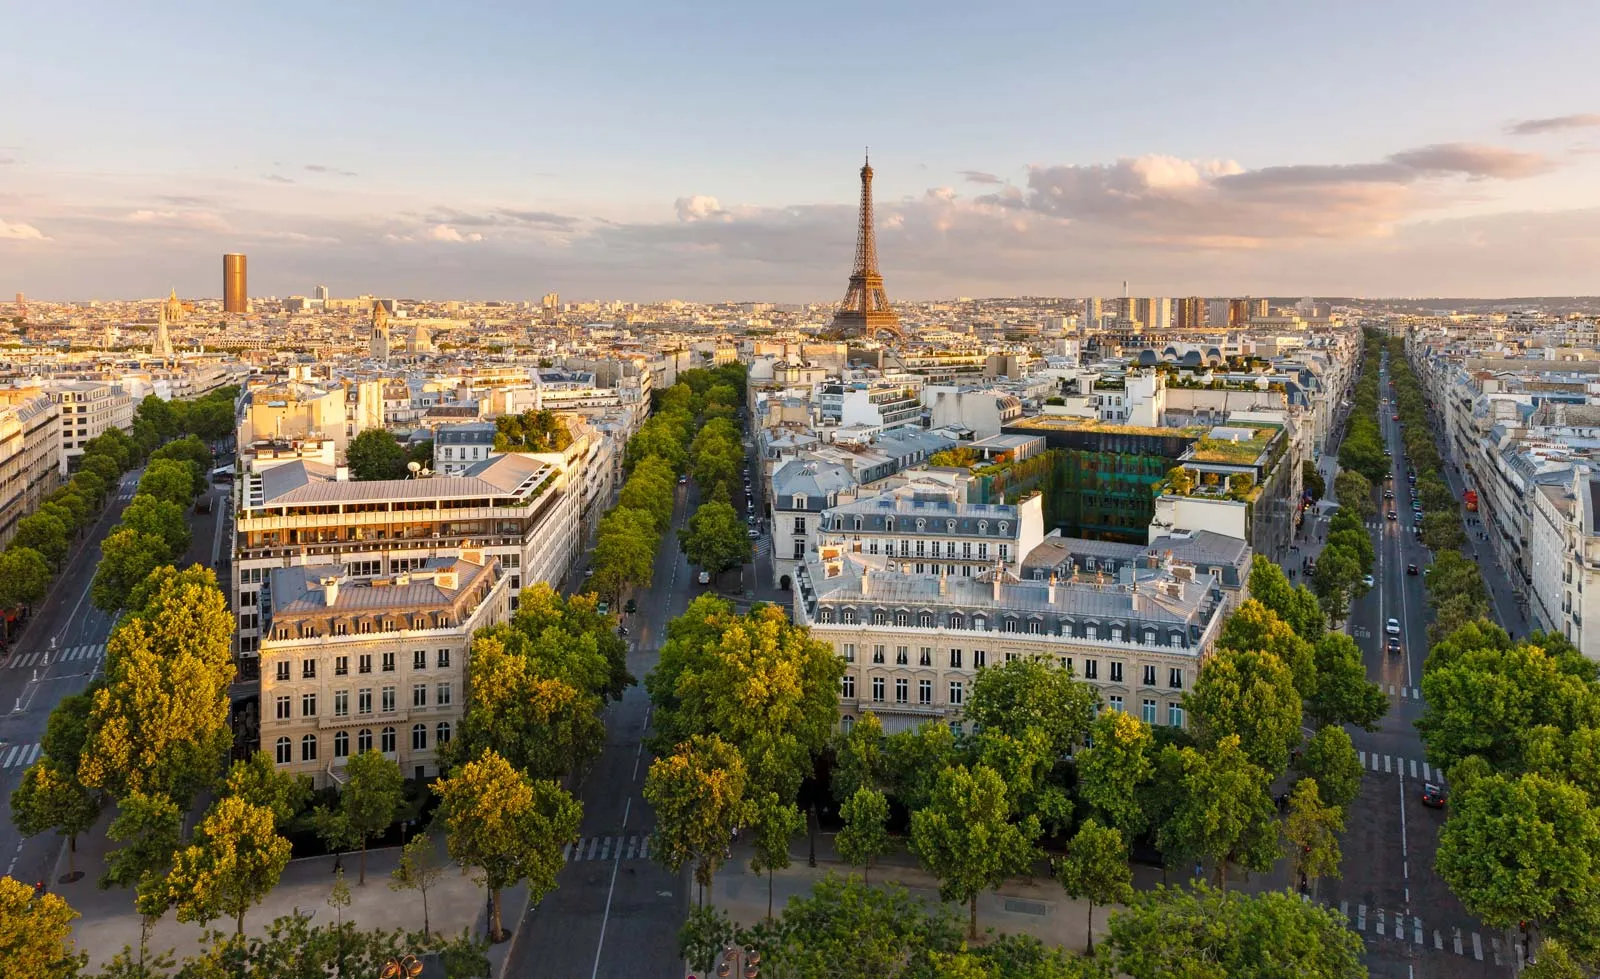
\includegraphics[height=5cm, keepaspectratio]{images/iledefrance.png}
                \caption{Picture of Paris in Île-de-France \cite{iledefrance}}
            \end{figure}
        \end{center}
        % Open source traffic demand generation pipeline
        % Samples population from real world french data
    \end{frame}
    
    \section{Graph Theory}
    
    \begin{frame}{Example Graph}
        \begin{center}
            \begin{figure}
                \centering
                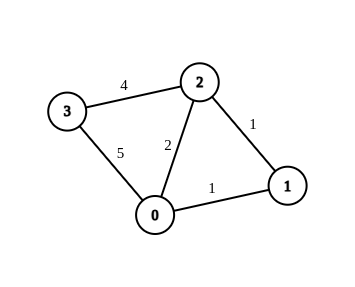
\includegraphics[height=5.5cm, keepaspectratio]{images/graph.png}
                \caption{Graph with nodes and edges \cite{graphs}}
            \end{figure}
        \end{center}
        % This is a graph with edges and nodes
    \end{frame}
    
    \begin{frame}{Minimum Spanning Tree}
        \begin{center}
            \begin{figure}
                \centering
                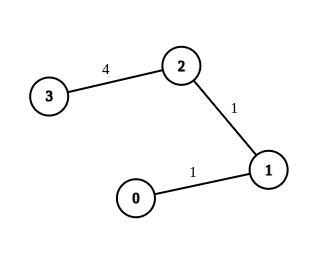
\includegraphics[height=5.5cm, keepaspectratio]{images/mst.png}
                \caption{Minimum Spanning Tree of Previous Graph \cite{graphs}}
            \end{figure}
        \end{center}
        % This is the minimum spanning tree of the original graph
        % The sum of the weights on the edges is minimum and there are no cycles created
        % This is a spanning tree also because all the nodes are connected
    \end{frame}
    
    \begin{frame}{Depth First Search}
        \begin{center}
            \begin{figure}
                \centering
                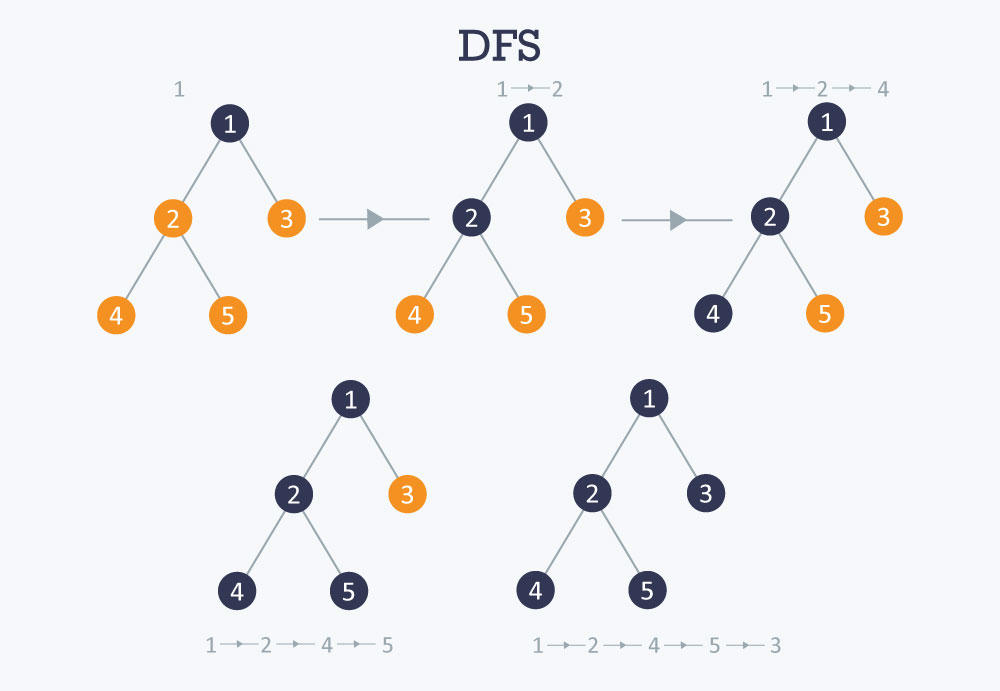
\includegraphics[height=5.5cm, keepaspectratio]{images/depthfirstsearch.jpg}
                \caption{Depth First Search Algorithm \cite{depthfirstsearch}}
            \end{figure}
        \end{center}
        % This is a technique to search through a graph
        % The search goes down a route till it finds that it has reached a node with no unvisited neighbors
        % The search then backtracks to the last node visited with an unvisited neighbor
    \end{frame}
    
    % MATSIM
    
    \section{Zoning}
    
    \begin{frame}[fragile]{Types of Zoning}
        \begin{figure}
            \centering
            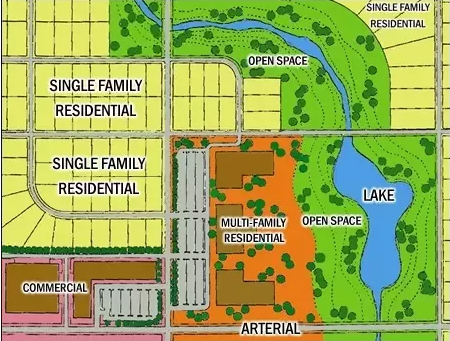
\includegraphics[height=5cm, keepaspectratio]{images/zoning.png}
            \caption{Example Zoning Structure \cite{zoningdiagram}}
        \end{figure}
        % Euclidean Zoning
            % Hierarchical
            %Flat (Non Hierarchical)
        % Performance Based (Point System
        % Form Based
    \end{frame}
    
    \begin{frame}[fragile]{Iteration One}
        \begin{center}
            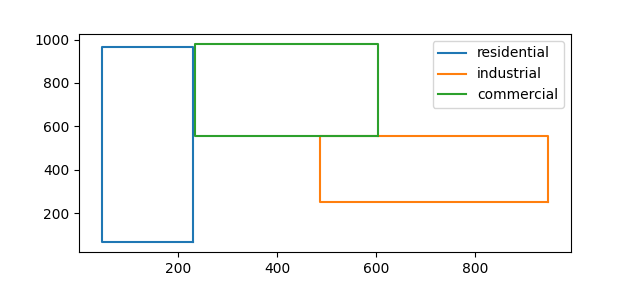
\includegraphics[height=5cm, keepaspectratio]{images/first-zoning.png}
        \end{center}
        % This iteration of zoning had individual boxes that were very intensive to compute
        % The space was also not completely utilized
    \end{frame}
    
    \begin{frame}[fragile]{Iteration Two}
        \begin{center}
            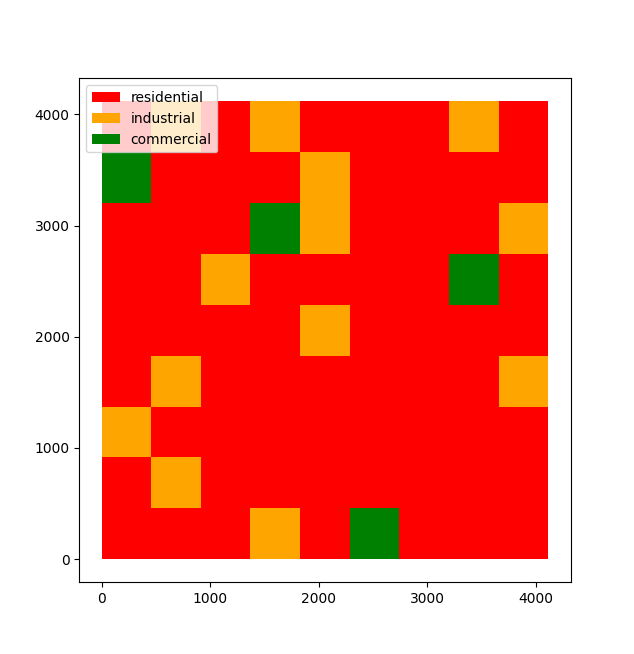
\includegraphics[height=6.6cm, keepaspectratio]{images/secondzoning.png}
        \end{center}
        % This iteration of the zones used a grid system to divide up all the space, but the different boxes had no relation to one another
    \end{frame}
    
    \begin{frame}{Connecting Regions}
        \begin{center}
            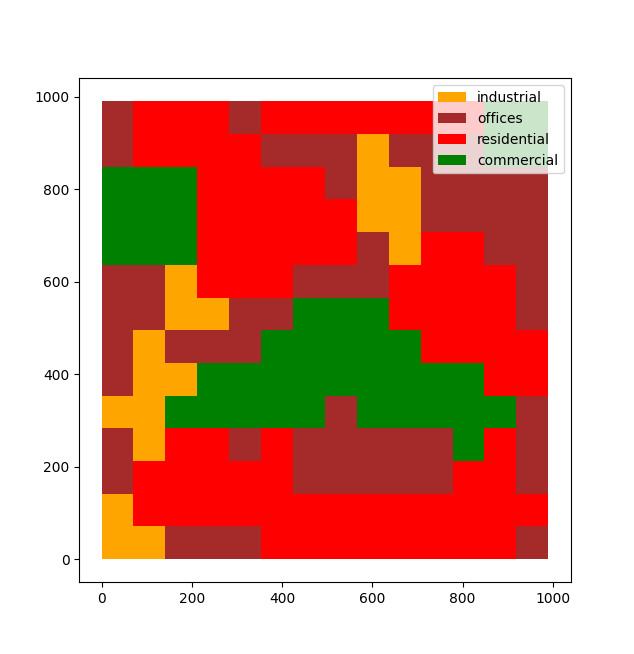
\includegraphics[height=6.6cm, keepaspectratio]{images/finalzoning.png}
        \end{center}
        % Cellular automata was considered for connecting regions, but depth first search was later chosen as a better alternative
        % This final iteration of zoning incorporated depth first search to create larger regions called districts out of the little cells on the grid
        % The size of the cell was set to the size off the largest building in any given zone (This is technically a limitation)
    \end{frame}
    
    \section{Network}
    
    \begin{frame}{First Iteration}
        \begin{center}
            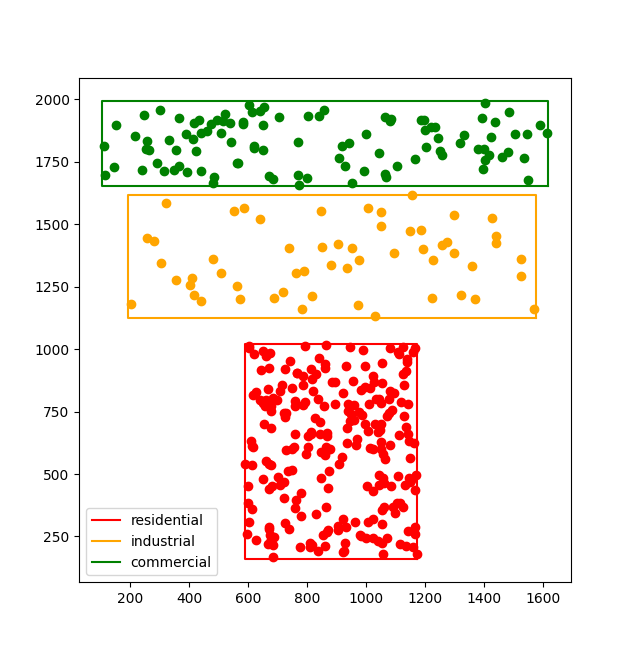
\includegraphics[height=6.6cm, keepaspectratio]{images/firstzoningwnodes.png}
        \end{center}
        % This first iteration of the network was with the first zoning model that only included nodes
        % The network did not contain roads yet...
    \end{frame}
    
    \begin{frame}{Second Iteration}
        \begin{center}
            \begin{tabular}{cl}
                \begin{tabular}{c}
                    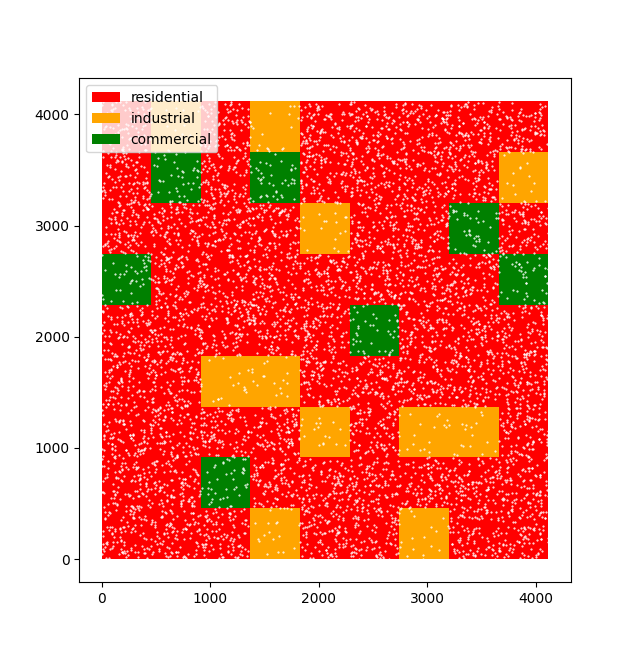
\includegraphics[height=5.2cm, keepaspectratio]{images/secondzoningwnodes.png}
                \end{tabular}
                 
                \begin{tabular}{l}
                    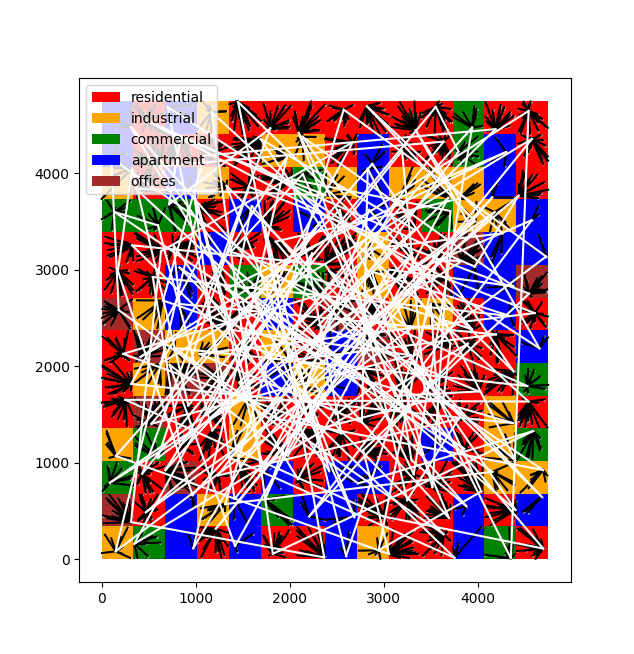
\includegraphics[height=5.2cm, keepaspectratio]{images/secondzoningwnetwork.png}
                \end{tabular}
            \end{tabular}
        \end{center}
        % This iteration of the network contained configurable number of nodes within each block
        % There was also a very inefficient road system on top of these nodes (no graph theory yet)
    \end{frame}
    
    \begin{frame}{Final Iteration}
        \begin{center}
            \begin{tabular}{cl}
                \begin{tabular}{c}
                    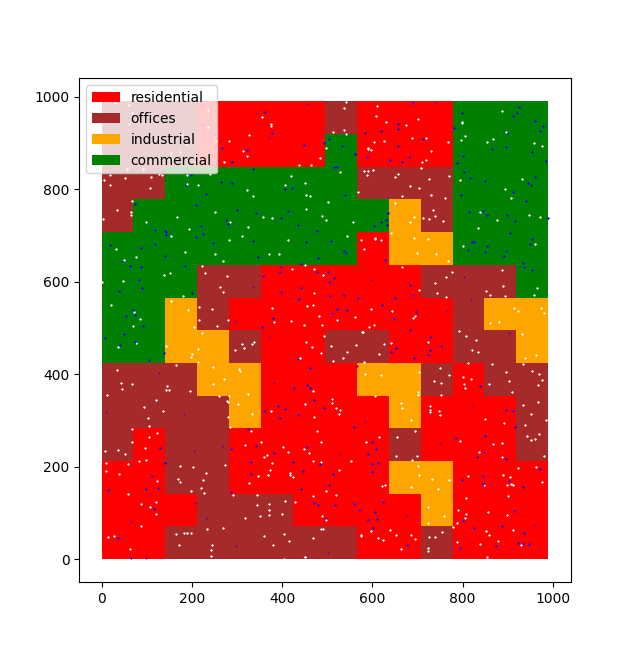
\includegraphics[height=5.2cm, keepaspectratio]{images/finalzoningwnodes.png}
                \end{tabular}
                 
                \begin{tabular}{l}
                    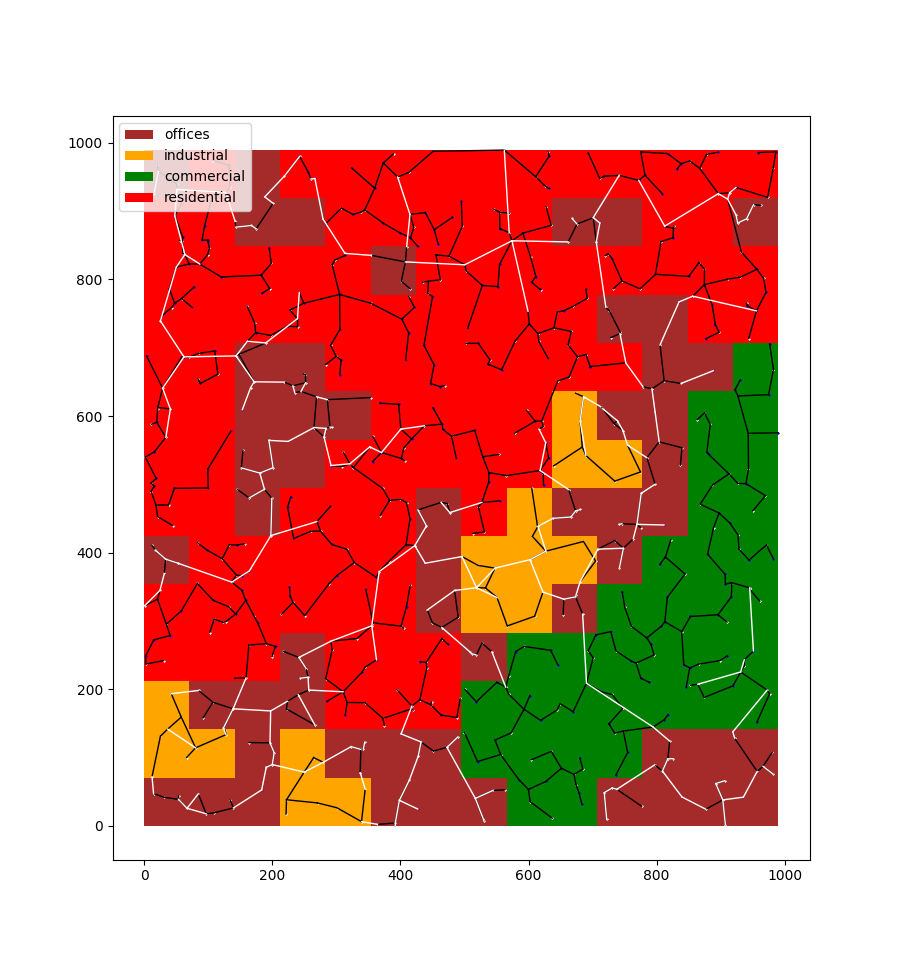
\includegraphics[height=5.2cm, keepaspectratio]{images/finalnetwork.png}
                    % Added subzones (hierarchy)
                \end{tabular}
            \end{tabular}
        \end{center}
        % The final iteration of the network included subzone nodes (a subzone node, such as an apartment in a commercial complex would only be added after atleast one commercial building was added to the district)
        % It also incorporated a minimum spanning tree to connect the roads in a much more efficient manner
    \end{frame}
    
    \begin{frame}{Meshing}
        \begin{center}
            \begin{figure}
                \centering
                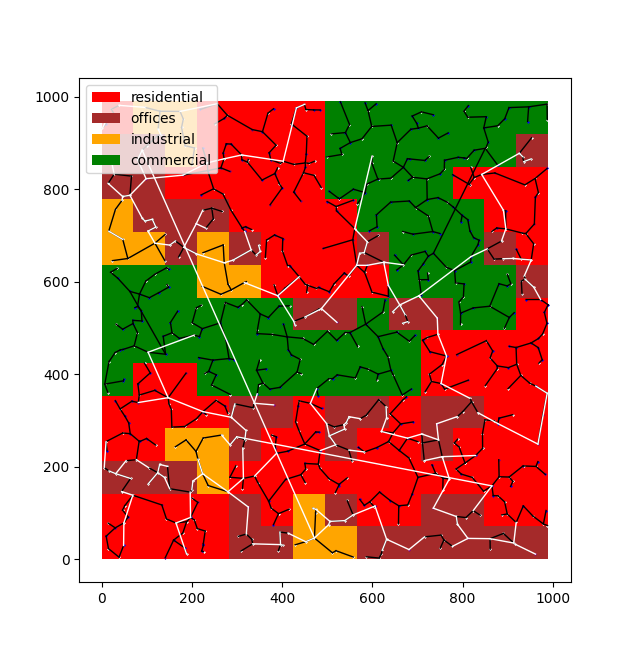
\includegraphics[height=5.5cm, keepaspectratio]{images/meshednetwork.png}
                \caption{1\% Meshed Network Example}
            \end{figure}
        \end{center}
        % The meshing ratio determines the number of remaining roads in the complete graph that are added to the minimum spanning tree to create the road network
        % Meshing ratio * number of roads in the minimum spanning tree = number of roads added
    \end{frame}
    
    \section{Agents}
    
    \begin{frame}{Example Population}
        \begin{columns}[T,onlytextwidth]
        
        \column{0.3\textwidth}
    
            \metroset{block=fill}
        
            \begin{block}{Activity}
            Work\\
            \vspace{1em}
            Leisure 0\\
            \vspace{1em}
            Leisure 1\\
            \vspace{1em}
            Leisure 2\\
            \vspace{1em}
            \end{block}
    
        \column{0.35\textwidth}
    
            \metroset{block=fill}
        
            \begin{alertblock}{Timings}
            9 AM - 5 PM\\
            \vspace{1em}
            5 PM - 8 PM\\
            \vspace{1em}
            8 PM - 10:30 PM\\
            \vspace{1em}
            10:30 PM - 11PM\\
            \vspace{1em}
            \end{alertblock}
    
        \column{0.35\textwidth}
    
            \metroset{block=fill}
    
            \begin{exampleblock}{Location}
                (827, 959)\\
                \vspace{0.92em}
                (774, 719)\\
                \vspace{0.92em}
                (707, 846)\\
                \vspace{0.92em}
                (647, 464)\\
                \vspace{0.92em}
            \end{exampleblock}
            
        \end{columns}
        % The program also generates schedules for every member in the population including the vehicles they use to get everywhere
        % Every activity is determined by the zones and a building in a zone can be given activity times for different types, such as work, leisure, and even residential (people can throw parties at their homes)
    \end{frame}
    
    \section{Let's Build a City}
    % The following section is data from an example city we will build together
    % If the program is run as a whole, only the whole network is shown, so to show the individual parts of the city, the program must be run several times
    % To allow for the same zoning and nodes every time the program is run to create the different parts of the city, the program also has configurable random seeds for each part of the city
    
    \begin{frame}{Zones}
        \begin{center}
            \begin{figure}
                \centering
                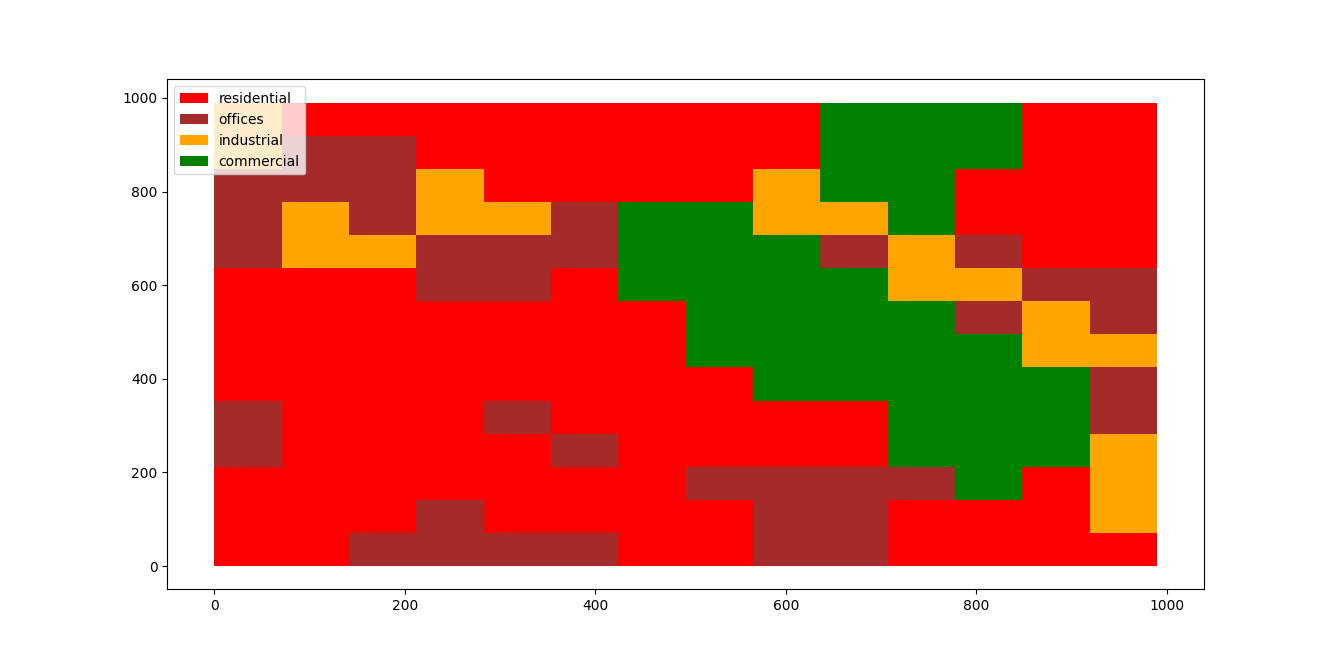
\includegraphics[height=5cm, keepaspectratio]{images/build_city/zones.png}
                \caption{50\% Residential, 10\% Industrial, 20\% Commercial, 20\% Offices}
            \end{figure}
        \end{center}
    \end{frame}
    
    \begin{frame}{Nodes}
        \begin{center}
            \begin{figure}
                \centering
                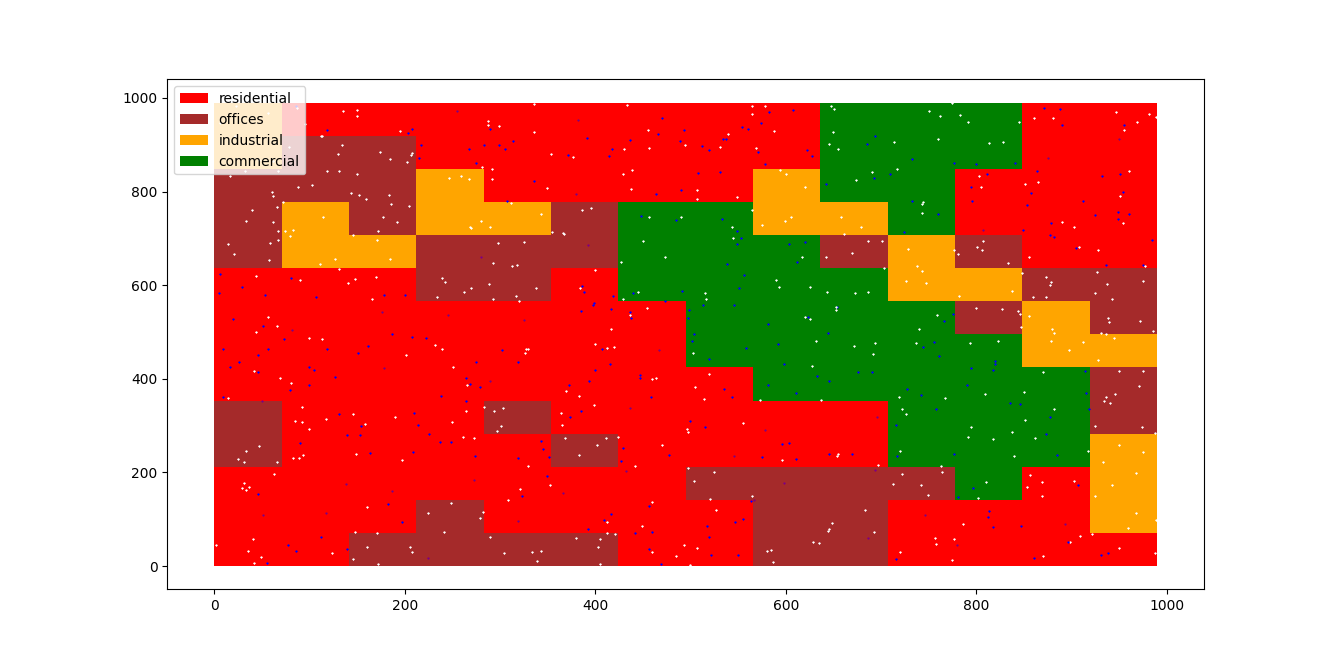
\includegraphics[height=5cm, keepaspectratio]{images/build_city/nodes.png}
                \caption{Subzones: Schools, Apartments; Building Sizes Based on Austin}
            \end{figure}
        \end{center}
    \end{frame}
    
    \begin{frame}{Network}
        \begin{center}
            \begin{figure}
                \centering
                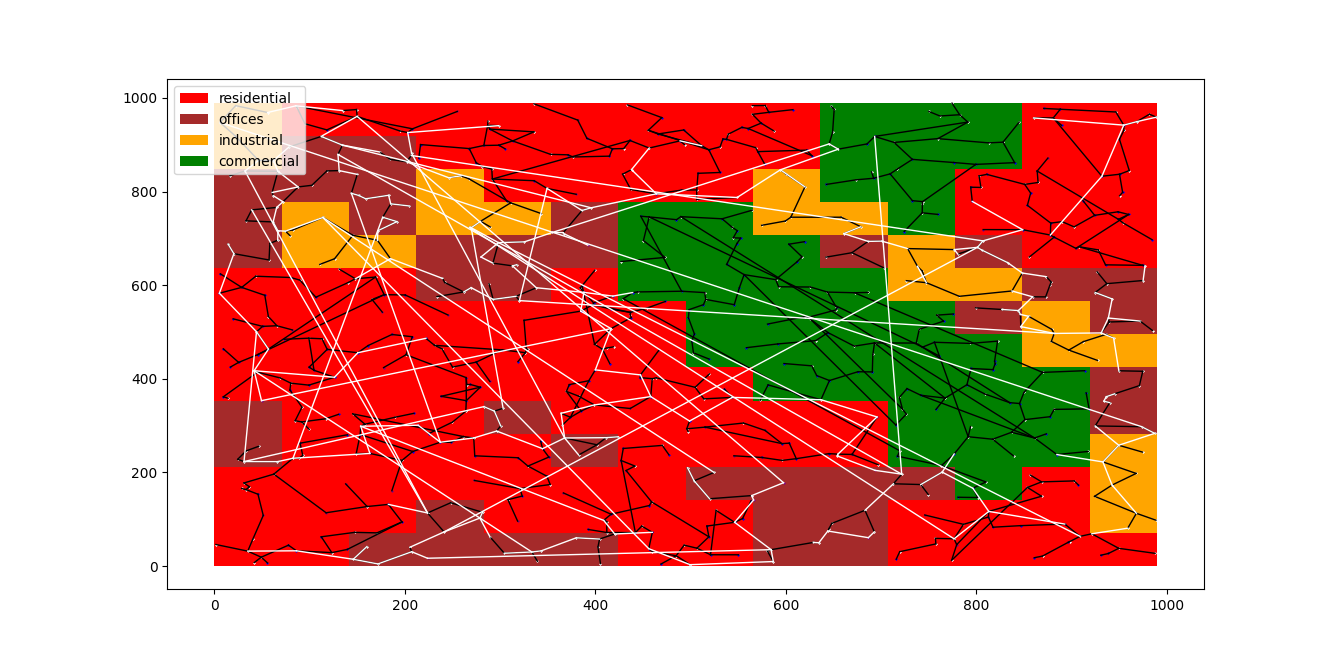
\includegraphics[height=5cm, keepaspectratio]{images/build_city/links.png}
                \caption{Meshing Ratio 10\%}
            \end{figure}
        \end{center}
    \end{frame}
    
    \begin{frame}{Population}
        \begin{center}
            \Huge This city has \texttt{\textbf{36,370}} people in it
        \end{center}
    \end{frame}
    
    \begin{frame}{Compare to Austin}
        \begin{center}
            \begin{figure}
                \centering
                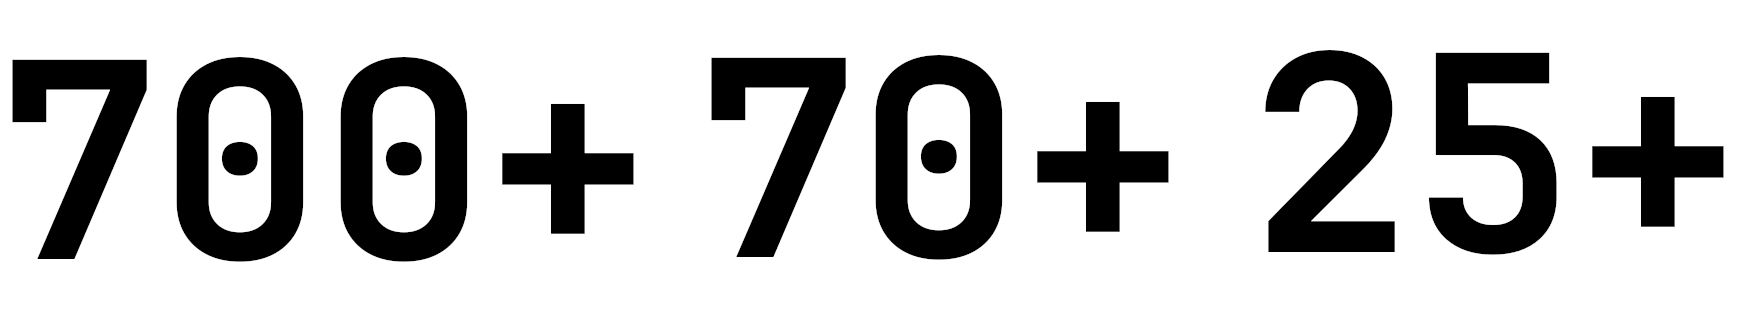
\includegraphics[height=2cm, keepaspectratio]{images/build_city/stats.png}
                \caption{700 times as much land, 70 times as many miles of roads, and 25 times lane miles of road as Austin}
            \end{figure}
        \end{center}
    \end{frame}
    
    \begin{frame}{Results i}
        \begin{center}
            \begin{figure}
                \centering
                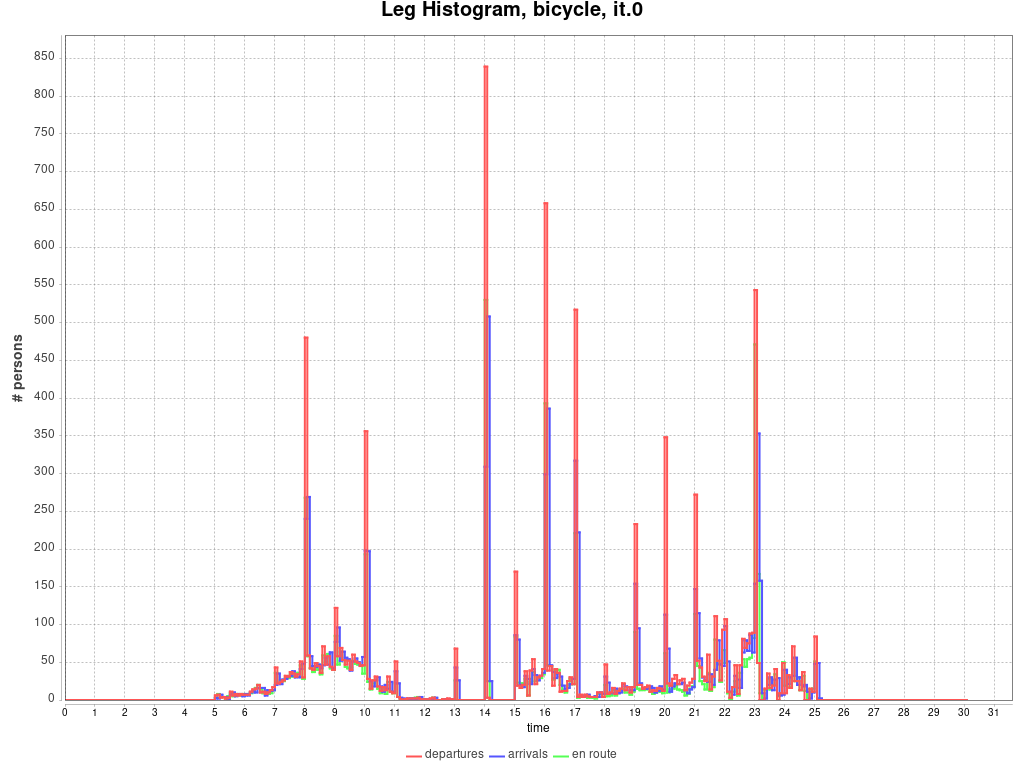
\includegraphics[height=6cm, keepaspectratio]{images/build_city/results/0.legHistogram_bicycle.png}
            \end{figure}
        \end{center}
    \end{frame}
    
    \begin{frame}{Results ii}
        \begin{center}
            \begin{figure}
                \centering
                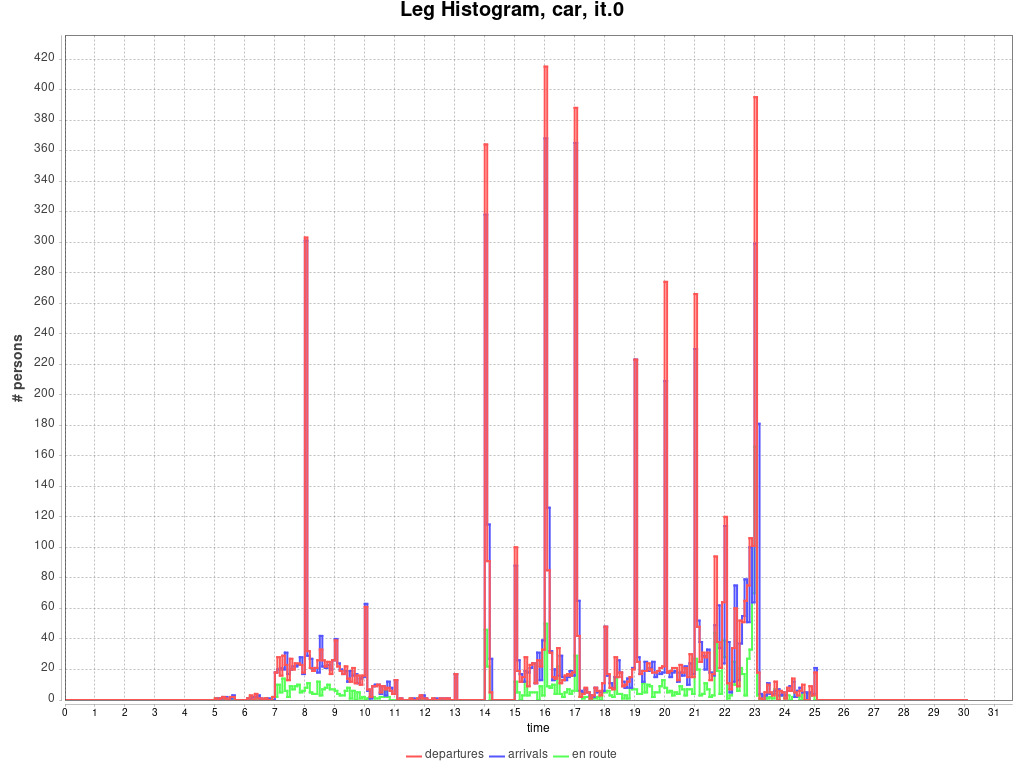
\includegraphics[height=6cm, keepaspectratio]{images/build_city/results/0.legHistogram_car.png}
            \end{figure}
        \end{center}
    \end{frame}
    
    \begin{frame}{Results iii}
        \begin{center}
            \begin{figure}
                \centering
                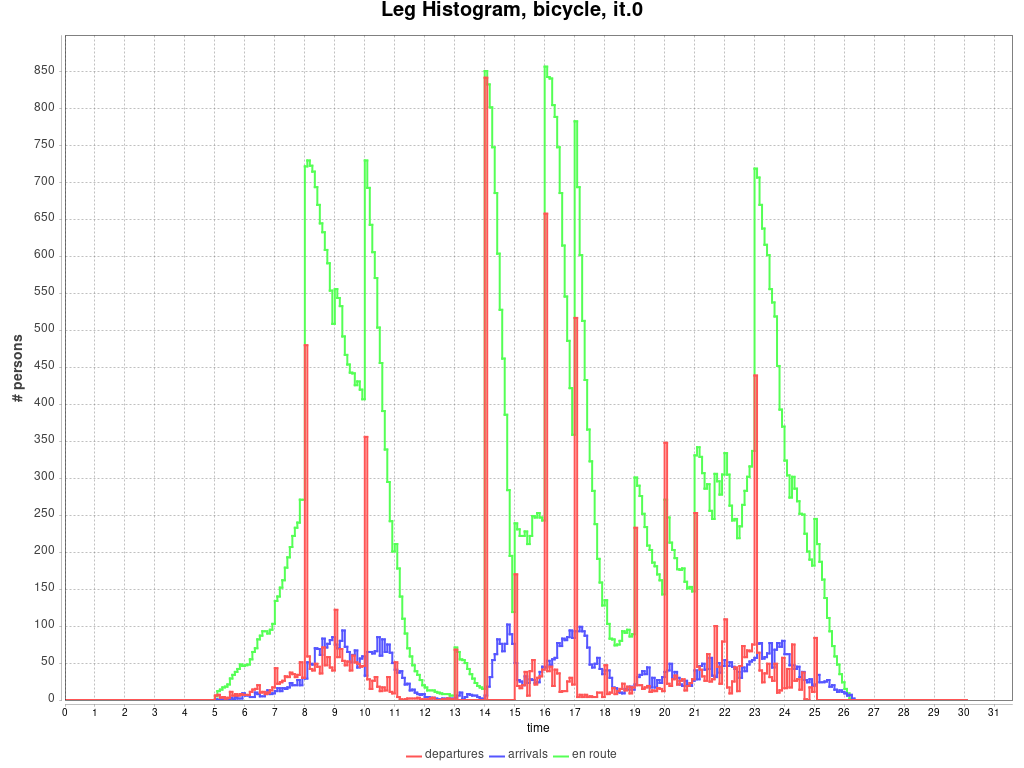
\includegraphics[height=6cm]{images/build_city/results/0.legHistogram_slow_bicycle.png}
            \end{figure}
        \end{center}
    \end{frame}
    
    \begin{frame}{Results iv}
        \begin{center}
            \begin{figure}
                \centering
                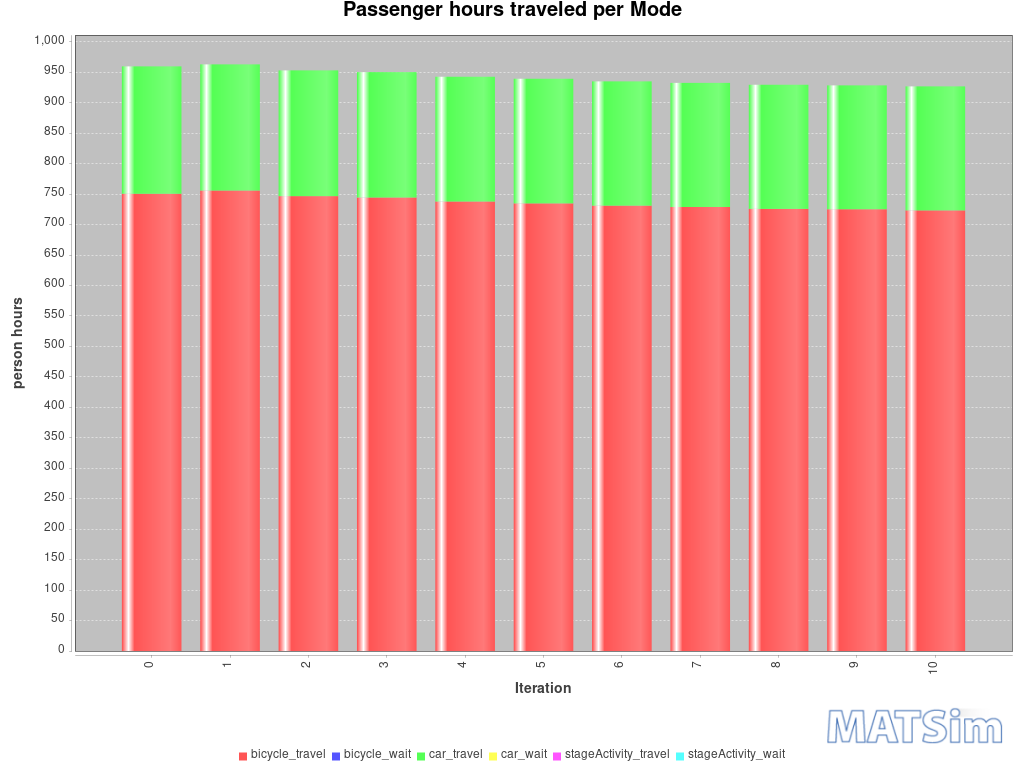
\includegraphics[height=6cm, keepaspectratio]{images/build_city/results/ph_modestats.png}
            \end{figure}
        \end{center}
    \end{frame}
    
    \begin{frame}{Results v}
        \begin{center}
            \begin{figure}
                \centering
                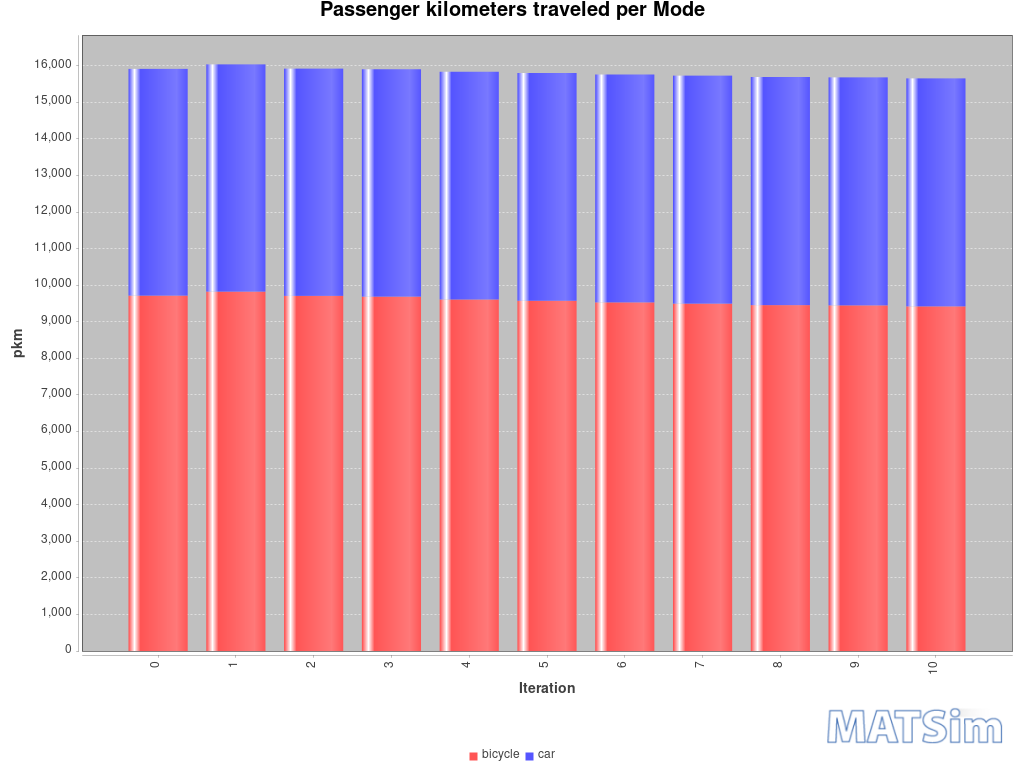
\includegraphics[height=6cm, keepaspectratio]{images/build_city/results/pkm_modestats.png}
            \end{figure}
        \end{center}
    \end{frame}
    
    \section{Conclusion}
    
    \begin{frame}{What's Next?}
        % The next step would include adding multiple modes of transport that can be used interchangebly during one leg.
        % Addition of EVs to the system could open the doors to simulating carbon emissions from city layouts as well...
        % The ceiling is endless we can keep adding configurations till we capture the most specific details. However, I believe that the place the project has gotten to today represents a city fairly holisticly and can thus reveal wonders about our world today.
        \begin{figure}
            \centering
            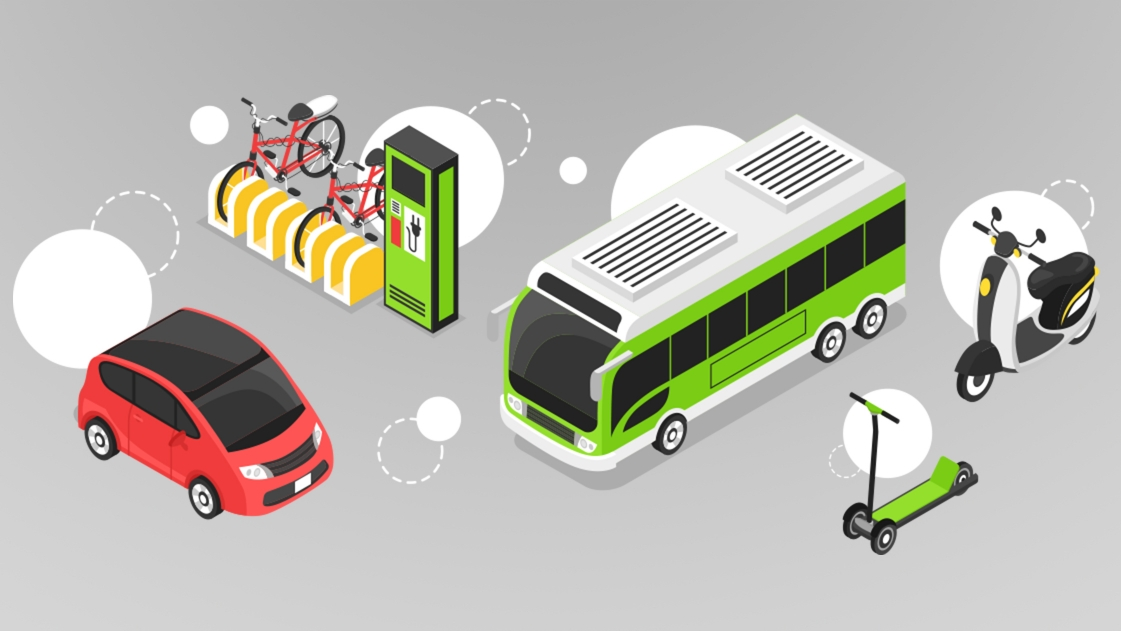
\includegraphics[height=5cm, keepaspectratio]{images/multimodaltransport.jpg}
            \caption{Multi-modal Transportation \cite{multimodal}}
        \end{figure}
    \end{frame}
    
    \section{Questions}
    
    \begin{frame}[allowframebreaks]{References}
        \bibliography{bibliography}
        \bibliographystyle{abbrv}
    \end{frame}

\end{document}
